\documentclass{article}
\usepackage[left=0.5in,top=0.5in,right=0.5in,bottom=0.5in]{geometry}
\usepackage[english]{babel}
\usepackage[utf8]{inputenc}
\usepackage[table]{xcolor}
\usepackage{amssymb,amsmath,amsthm}
\usepackage{changepage,threeparttable}
\usepackage{booktabs,multirow}
\usepackage{graphicx}
\usepackage{soul}
\graphicspath{{./images/}}
\def\F#1{\(#1\)}
\title{Lab 11: Electron Acceleration and Deflection by Electrostatic Fields}
\author{Philip Kim}
\date{\today}
\begin{document}
\maketitle
\vspace*{-1cm}
\begin{table}[!htp]\centering
  \begin{tabular}{|c|c|c|c|}\hline
    \multicolumn{4}{|c|}{\textbf{Table 2: Electron Deflection}}\\\hline
    \F{X_{obs}}&\F{Y_{obs}}&Y&\F{F_D}\\\hline
    8.3&-2.40, 2.35&2.38&-0.03\\\hline
    8.0&-2.20, 2.05&2.13&-0.08\\\hline
    7.3&-2.10, 1.45&1.78&-0.33\\\hline
    7.0&-1.40, 1.35&1.38&-0.03\\\hline
    6.3&-1.30, 1.25&1.28&-0.03\\\hline
    6.0&-1.20, 1.15&1.18&-0.03\\\hline
    5.3&-1.10, 1.10&1.10&0.00\\\hline
    5.0&-0.50, 1.00&0.75&0.25\\\hline
    4.3&-0.40, 0.50&0.45&0.05\\\hline
    4.0&-0.30, 0.30&0.30&0.00\\\hline
  \end{tabular}
\end{table}
\begin{itemize}
  \item[(a)] Measure the distance between the plates s = \F{\boxed{5.3~cm}}
  \item[(b)] Graph \F{y~vs.~x^2}, include error bars. Measure the slope of the graph, slope =?
  \item[] b
  \item[(c)] From the slope, calculate the correction factor \F{F_D=?}
  \item[] c
\end{itemize}
\newpage
\begin{table}[!htp]\centering
  \begin{tabular}{|c|c|c|c|c|}\hline
    \multicolumn{5}{|c|}{\textbf{Table 3: Thompson's Experiment}}\\\hline
    \F{V_{PS} (kV)}&2.00&2.50&3.00&3.50\\\hline
    \F{I} (A)&0.18&0.23&0.28&0.33\\\hline
    \F{B} (T)&7.62e-4&9.73e-4&0.12e-2&0.14e-2\\\hline
    \F{e/m} (C/kg)& & & & \\\hline
  \end{tabular}
\end{table}
Sketch the path of the beam:\\
\fbox{\begin{minipage}{53em}
  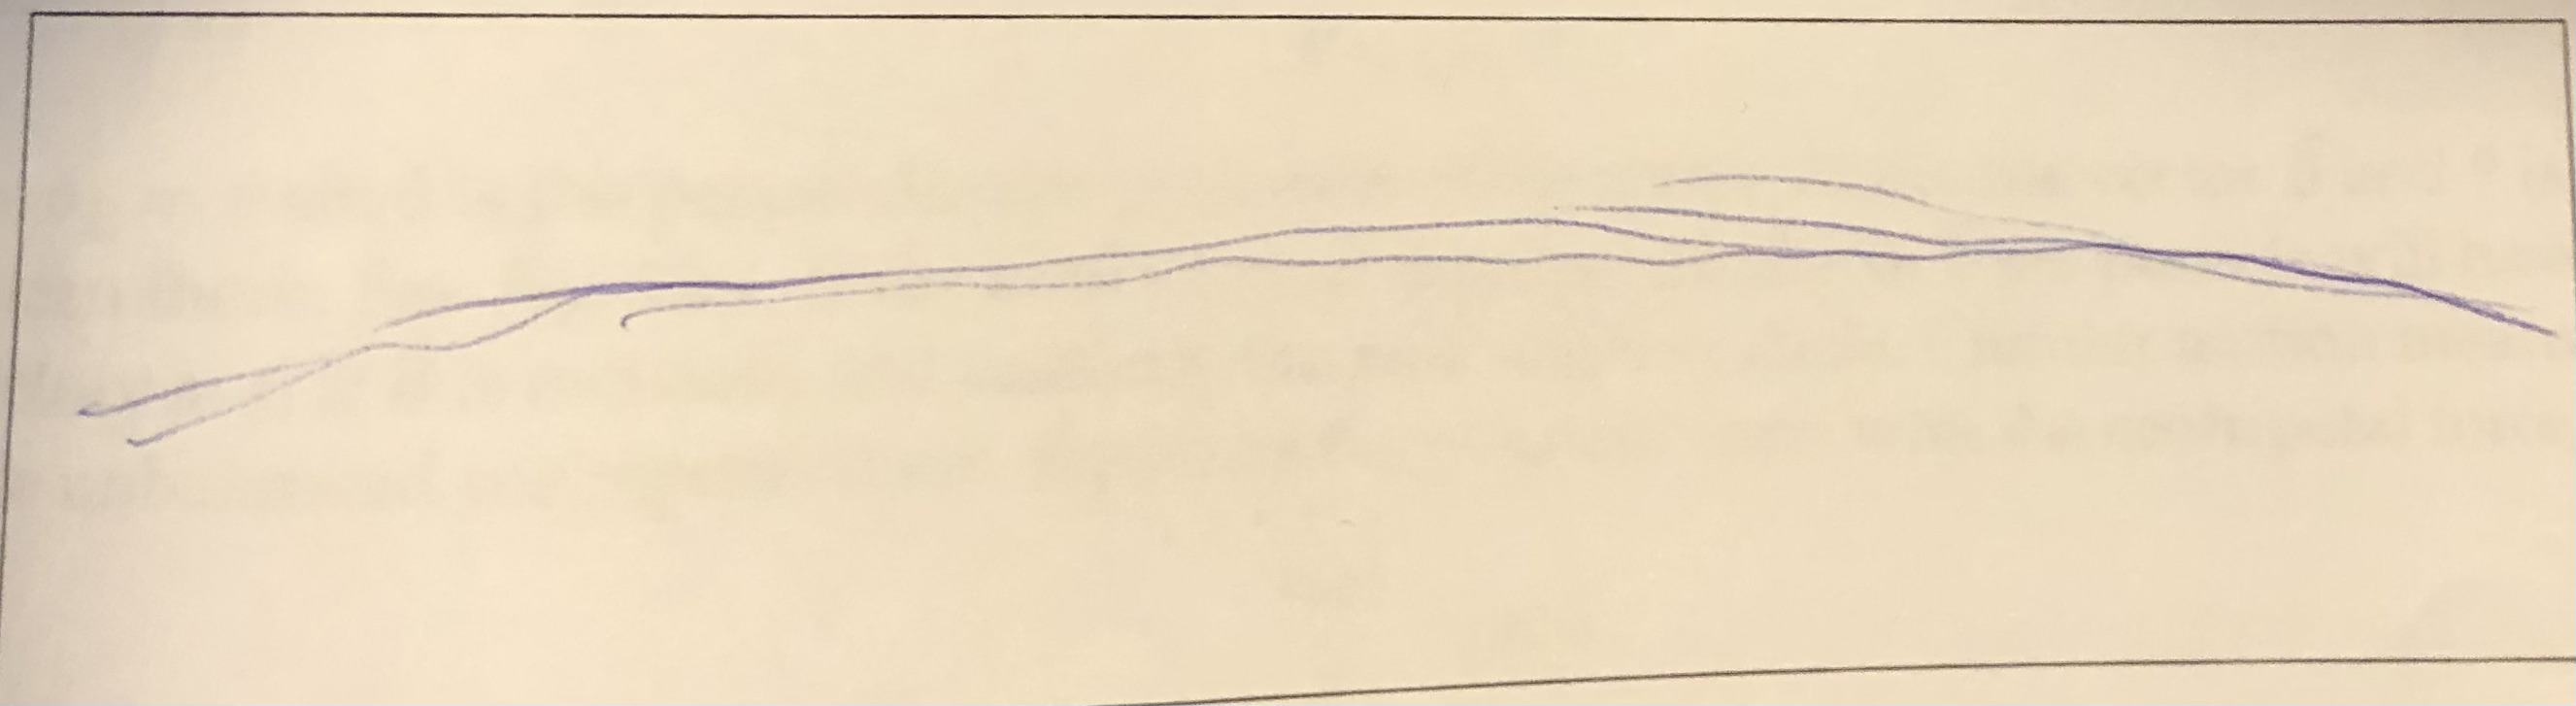
\includegraphics[width=\textwidth]{beam.jpeg}
\end{minipage}}
\subsection*{11.6 Questions}
\begin{enumerate}
  \item Calculate the speed of the electron for the maximum voltage available for acceleration, in meters per seconds.
  \item What fraction of the speed of light is this?
  \item According to the special theory of relativity, the mass m of an object that is moving with velocity v with respect to an observer is larger than its rest mass \F{m_0}. The rest mass is the mass of the object when it is at rest. The equation that describes this phenomenon is \begin{center}\F{m=\frac{m_0}{\sqrt{1-\frac{v^2}{c^2}}}},\end{center} where \F{c=3.0\times10^8m/s} is the speed of light in vacuum. Evaluate the mass for the electrons in this experiment that are moving at v you calculated in 1. How much larger is this than \F{m_0}?
  \item Compare your measured \F{e/m} from Thompsons Experiment to the known value, \F{1.76\times10^{11}C/kg}.
\end{enumerate}
\end{document}
